\documentclass[20pt]{article}

\usepackage{lmodern}

\usepackage[document]{ragged2e}
\usepackage{fancyhdr}
\usepackage{graphicx}
\graphicspath{Images}
\pagestyle{fancy}
\fancyhf{}
\lhead{Compiler Chapter 2 Notes}
\rhead{Daniel Lee}

\rfoot{Page \thepage}
\title{Chapter 2}
\author{Daniel Lee}
\date{May 7th,  2022}
\begin{document}
\maketitle
\newpage
\justify
\section*{Introduction}
    \begin{itemize}
        \item A compiler scans an input of characters and outputs a stream of words labelled by syntatic category
        \item A microsyntax is used to group words that have meaning within the source language  
        \item Some words such as keywords have special meaning, which makes them reserved 
        \item An example of this would be the \textit{while} and \textit{static} keywords in the Java programming language
        \item To recognize keywords, the scanner can either use dictionary lookup or encode keywords directly into microsyntax
        \item The simple lexical structure of programming languages lends itself to efficent scanners
    \end{itemize}
\section*{Recognizing Words}
    \begin{itemize}
        \item When we are parsing words we can view the parsing process as a series of if-else statements or a state machine 
        \item Transition diagrams often provide a simple means of formalizing the abstractions a compiler may need to implement them
        \item S is the finite set of states in the recognizer, alongside with error state $s_e$
        \item $\Sigma$ is the finite alphabet recognized by the recognizer 
        \item $\delta(s,c)$ is the transition function, it maps the value of state s and c,into some state
        \item In state $s_i$ with transition character $c$, the state makes the following transition $s_i \rightarrow_c \delta(s_i,c)$
        \item $s_0 \in S$ refers to initial state
        \item $S_a (S_a \subseteq S)$, is the set of accepting states
    \end{itemize}
    \subsubsection*{Example:}
    $S = \{s_0, s_1, s_2, s_3, .......,s_10,s_e\}\\
    \Sigma = \{ e, h, i, l, n, o, t, w\} \\
    \delta = \\
        \begin{cases}
        s_0 \rightarrow_n s_1, s_0 \rightarrow_w s_6, s_1 \rightarrow_e s_2, s_1 \rightarrow_o s_4, s_2 \rightarrow_w s_3 
        \\s_4 \rightarrow_t s_5, s_6 \rightarrow_h s_7, s_7 \rightarrow_i s_8, s_8 \rightarrow_l s_9, s_9 \rightarrow_e s_{10} 
        \end{cases}\\
        s_0 = s_0\\
        S_A = \{s_3,s_5,s_{10}\}\\
    $

    \newpage
\subsection*{More complex words:}
        \begin{itemize}
            \item For more complex words we can have the state machine accept multiple inputs
            \item We can vastly simplify state machines by using cycles
        \end{itemize}
        \subsubsection*{Practice Problems:}
            \begin{itemize}
                \item Problem 1: A six-character identifier consisting of alphanumeric characters followed by zero to five-alpha numeric characters
                    \begin{itemize}
                        \item $S = \{s_0, s_1,s_e\}$ 
                        \item $\Sigma = {a = \textbf{set of all-alphabet},b = \textbf{set of all alphanumeric}}$
                        \item $s_0 = s_0$
                        \item $\delta = \begin{cases}
                            s_0 \rightarrow_a s_1, s_{1} \rightarrow_b s_{1}
                        \end{cases}$
                        \item $S_A = {s_1}$
                    \end{itemize}
                \item Problem 2: 
                    \begin{itemize}
                        \item $S = \{s_0, s_1,s_2 s_e\}$
                        \item $\Sigma  = {(,)}$
                        \item $s_0 = s_0$
                        \item $S_A = \{s_2\}$
                        \item $\delta = \begin{cases}
                            s_0\rightarrow_{(} s_1, s_1 \rightarrow_{)} s_2, s_2 \rightarrow_{(} s_1 \} 
                        \end{cases}$
                    \end{itemize}
                \item Problem 3: A Pascal comment which consists of \{, zero  or more characters from the alphabet, and closed by \}:
                  \begin{itemize}
                    \item $S = \{s_0, s_1,s_2\}$
                    \item $\Sigma = \{ \},\{,a...z,A...Z,0...9\}$
                    \item $s_0 = s_0 $
                    \item $S_A = \{S_3 \}$
                    \item $\delta = \begin{cases}
                        s_0 \rightarrow_{\{} s_1\\
                        s_1 \rightarrow_{(a...z,A...Z,0...9)} s_1\\
                        s_1 \rightarrow_\{ s_2
                    \end{cases}$
                  \end{itemize}
                  \end{itemize}
    \subsection*{Regular Expression}
                  \begin{itemize} 
                    \item The set of all words accepted by a finite automaton, F, forms a language L(F)
                    \item For any FA, we can describe describe the language using regular expression or RE
                    \item The language consists of single world "new" can be described as RE, new 
                    \newpage
                    \item A language consisting of two words, new or while can be represented as RE new$|$while
                    \item new or not can be represent by RE, n(ew$|$ot)
                    \item Let us consider the example of punctuation marks, a REs for punctuation may appear such as: : ; ? = $>$ ( ) {} []
                    \item Keywords may have an expression such as this: if while this integer instanceof
                    \item more complex RE: 0 $|(0|1|2|3|4|5|6|7|8|9) (0|1|2|3|4|5|6|7|8|9)*$
                    \item \textbf{The following operator is called a kleen operator and indicates there can be zero or more instances of a RE} 
                \end{itemize}
    \subsection*{Formalizing notes for regular expressions: }
                \begin{itemize}
                    \item Given a regular expression r, we can denote the Language it describes as L(r)
                    \item An RE is made up of 3 operations:
                    \item Alternation: The alternation or union of two sets R and S denoted R$|$S or \{$x|x \in R$ or $x \in S $\}  
                    \item Concatenation: The concatentation of two sets RS contains all strings formed by prependong an element of R onto one from S,
                    or \\\{xy$|x \in R \: and \: y \in S $\}
                    \item Closure: The kleene closue of a set R, denoted by $R^*$ is $\cup_{i = 0}^{\inf} R^i$ is a concantenation of R with itself zero or more times
                    \item Sometimes we can use notation for finite closure if a set is concantenated multiple times: \\
                    $(R|RR|RRR)$
                    \item Positive Closure is Denoted if $RR^*$
                    \begin{itemize}
                        \item If  $ a\in \Sigma$, then a is also an RE denoting set containing only a
			\item If r and s are RES, denoting sets L(r) and L(s) then r $|$ s is a RE denoting the union, or alternation of L(r) and L(s)\\
			Similarly rs is an RE denoting the concatenation of L(r) and L(s)\\
			$r^*$ is an RE denoting Kleene closure of L(r)
			\item $\epsilon$ represents a RE of an empty string
			\item Parentheses have the highest precedence, followed by closure, concatenaton, and alternation
                    \end{itemize}
		    \subsection*{Example:}
		    	\begin{itemize}
				\item Imagine a language in keywords start with a letter in the English alphabet and can be then followed by a sequence of alphanumeric
				character. We can represent the following keyword using RE: \\
				([A...Z]$|[a...z])([A..Z]|([a...z])|([0...9])^*$
				\item Let's consider another example one in which, we are representing unsigned integers:\\
				$(0|([1...9])([0...9])^*$
				\item Unsigned real number: \\
					$(0|([1...9])([1...9])^*)(\epsilon| .[0...9]^*)$
				\item Quoted strings using complement:\\
					A quoted String in a programing language is often composed of a " followed by ", in between these two characters any characters\\
					can appear. In theory we could write a regular expression that contains all the possible characters but this is impractical.
					To circumvent this issue we can use the complement operator:\\
					"$($\^{}"$)$"\\
                \item Comments can often appear in many forms:\\
                    $(//($ \^{}  $\backslash$n $)^*|$
                    $/*($ \^{}* $|$\^{}  */$)^* */)$
                 
                     
                \end{itemize}
			
                    \end{itemize}
            \subsection*{Closure properties of RE:}
                    \begin{itemize}
                        \item Many regular expressions are closed under many operations,i.e if we apply an operation to a RE we get a RE
                        \item Some obvious examples are concatenation, union, and closure
                        \item Imagine we have a collection of regular expressions to describe syntatic categories in a language: $a_0, a_1,...,a_n$
                        \item To describe all the valid words in a language we can use the RE: $a_0 | a_1 | a_2|...|a_n$
                        \item Closure under union suggests that any finite language is a regular language and can be arranged in alternation
                        \item Closure under concantentation also allows us to build complex REs from simpler one's by concatenating them 
                        \item REs are closed under complements
                    \end{itemize}
            \subsection*{Practice Problems: }
                    \begin{itemize}
                        \item Chapter 2: pg 42
                        \item Problem 1:
                        \item $a_0 = [A...Z], a_1 = [a...z], a_2 = [0...9]$
                        \subitem $(a_0|a_1)(a_0a_1a_2)^5$
                        \item Problem 2:
                        \item $a_0 = $\^{} "$, a_1 = "$
                        \subitem $a_1(a_0|a_1a_1)^*a_1$
                    \end{itemize}
            \section*{From Regular Expression to Scanner:} 
                    \begin{itemize}
                        \item Up to this point we have covered a decent amount of notation, so what is the point of all this notation
                        \item In this section we will be learning about deterministic FA(DFA) and nondeterministic FA(NFA) 
                    \end{itemize}
                    \subsection*{Nondeterministic Finite Automata}
                
                        \begin{itemize}
                            \item Recall that an empty string $\epsilon$ is a RE, but many FAs did not include the empty string within the state diagrams
                            \item So what role does $\epsilon$ play in  FA? 
                            \item The answer lies in using $\epsilon$ to build more complex state machines
                            \item For instance, we can use $\epsilon$ to represent concatentation of mn using $\epsilon$
				                    \subitem $\rightarrow s_0 \rightarrow_m s_1 \rightarrow_{\epsilon} s_2 \rightarrow_{n} s_3$
			                \item $\epsilon$ can often complicate how our model work
                                  \begin{itemize}
                                    \item Consider the following two FAs
                                    \begin{figure}[h]
                                    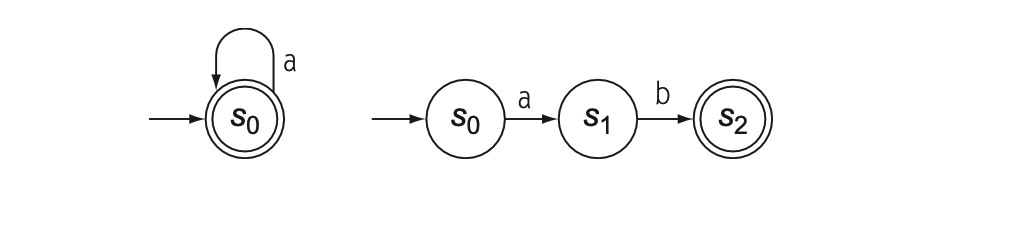
\includegraphics[width=\textwidth]{Images/uncombined.png}
                                    \end{figure}
                                    \newpage
                                    \item Utilizing the $\epsilon$ transition we can add complexity to our model to form $a^*ab$
                                    \begin{figure}[h]
                                        
\includegraphics[width=\textwidth]{Images/combined.png}
                                        \end{figure} 
                                    \item The following machine is called a NFA, due to the fact that for a specific character there can be transitions for same state depending on what character follows the input character 
                                    \item A DFA on the contrary can only have a single transition for a single character for a state
                            
                                  \end{itemize}
                        \subsubsection*{A Set of Models for NFA: }
                                  \begin{itemize}
                                      \item Each time a NFA makes a nondeterministic choice, it follows the transition  that transition that leads to accepting state of the input string
                                      \item Each time the NFA makes non-deterministic choice, it replicares itself to pursue each possible translation
                                      \item In this state, each possible translation is pursued and the current active state is called the \textit{configuration}
                                  \end{itemize}
                        \subsubsection*{Equivalence of  NFAs: }
                                  \item NFAs and DFAs are equivalent in their expressive power
                                  \item Any DFAs is a specical case of an NFA 
                                  \item Conversely any NFA can be emulated by a DFA
                                  \item Let us consider the state of a NFA when it has reached some point in input string
                                  \item If there are n states and $|\Sigma|$ character then by rule of product there are $|\Sigma|^n$ configurations
                                  \item To simulate the behavior of the NFA, we need a DFA for each configuration of NFA thus have more exponentially more states than NFA
                                  \item This can make a DFA expensive from space standpoint	
                                  \newpage	
                                  \item Examine the two figures below:		
                                  \begin{figure}[h]
                                    
\includegraphics[width=\textwidth]{Images/combined.png}
                                    
\includegraphics[width=\textwidth]{Images/nfaindfa.png}
                                  \end{figure}    
                                  \item Notice how both expressions are equivalent but instead of there of being two transition state for same characters
                                  one simply moves on to the next state and have self-loop
                        \end{itemize}
            \subsection*{Regular Expression to NFA: Thompson's Construction}
                        \begin{itemize}
                            \item Thompson's construction can be used to build NFA from RE
                            \item In a sense they are a template for building FAs and can be viewed as a combination of concatentation, alternation, and closure
                            \begin{figure}[h]
                                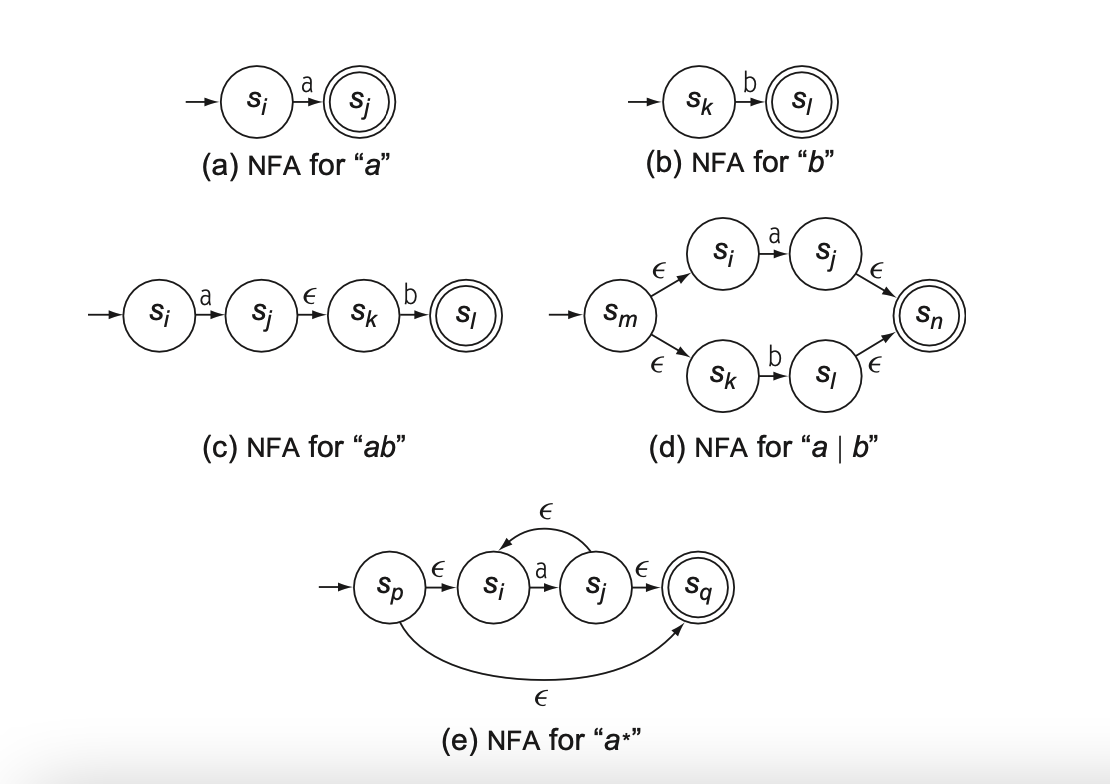
\includegraphics[width=\textwidth]{Images/thompson.png}
                            \end{figure}
                            \item The following FAs above are trivial RE that can be used to build much more complex state machines
                            \item The presence of one starting/accepting state makes the process of building a NFA much simpler 
                            \begin{figure}[h]
                                \includegraphics*[width=\textwidth]{Images/example.png}
                            \end{figure}
                            \item The following figure above represents a Thompson construction of $a(b|c)^*$
                        \end{itemize}
            \subsection*{NFA TO DFA: The Subset Construction}
                        \begin{itemize}
                            \item Thompson Construction produces an NFA to recognize the language specificatons of a RE
                            \item DFA execution is a lot simpler than NFA so having an algorithm to conver a Thompson construction to a DFA is useful
                            \item The resulting DFA are simpler and have several efficent implementations
                            \newpage
                            \item Below there shall be the algorithn for DFA construction using a NFA
                            \item The subset takes a NFA,($N, \Sigma, \delta_{N}, n_{0}, N_{A}$) and produces a DFA, ($D,\Sigma,\delta_{D}, d_{0}, D_{A} $
                            \begin{figure}[h]
                                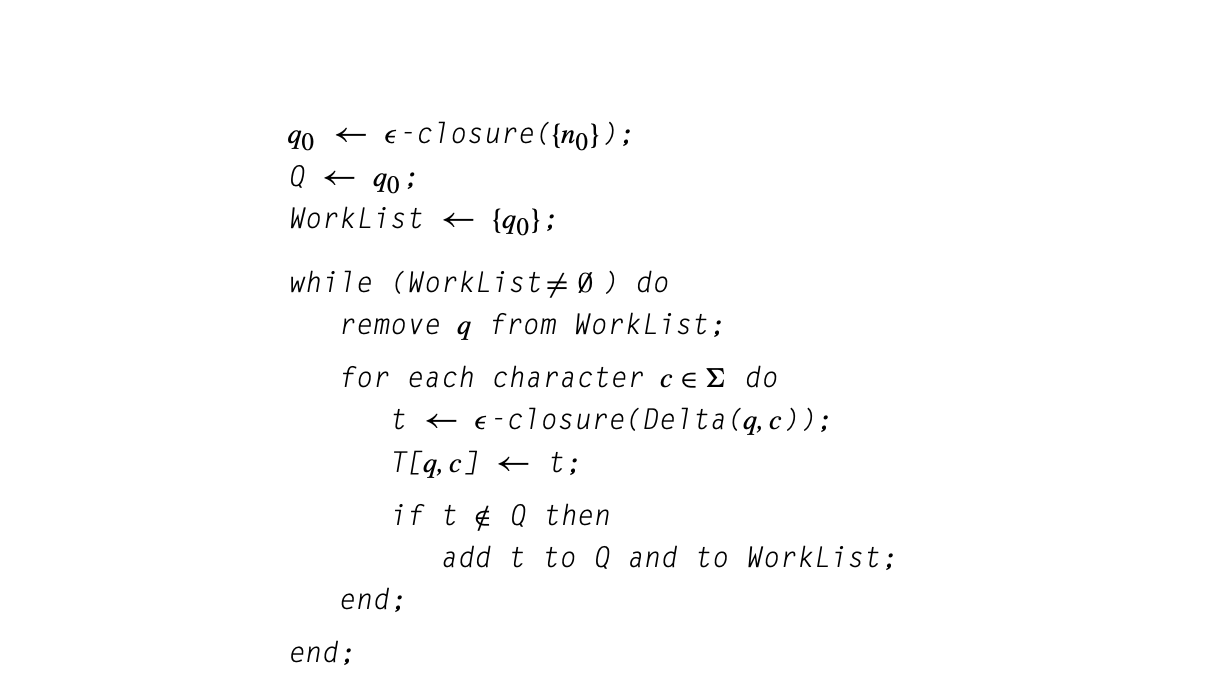
\includegraphics[width= \textwidth]{Images/subsetconstruction.png}
                            \end{figure}
                        \end{itemize}
\end{document}
